\documentclass[8pt,a4paper]{article}

\usepackage{amsmath, amssymb, amsthm}
\usepackage{tikz}
\usepackage{mathtools}
\usepackage{multicol}
\usepackage[top=0.5cm,left=0.5cm,right=0.5cm,bottom=0.5cm]{geometry}
\usepackage{amsfonts}
\usepackage{etoolbox}
\usepackage{cancel}
\usepackage{yhmath}
\usepackage{color}
\usepackage{hyperref}
\usepackage{cancel}
\usepackage{graphicx}
\usepackage{caption}
\usepackage[overload]{empheq} % For braced-style systems of equations.

\newenvironment{Figure}
  {\par\medskip\noindent\minipage{\linewidth}}
  {\endminipage\par\medskip}

\newenvironment{absolutelynopagebreak}
  {\par\nobreak\vfil\penalty0\vfilneg
   \vtop\bgroup}
  {\par\xdef\tpd{\the\prevdepth}\egroup
   \prevdepth=\tpd}

\definecolor{forestgreen(web)}{rgb}{0.13, 0.55, 0.13}
\definecolor{lavender(floral)}{rgb}{0.71, 0.49, 0.86}

\usepackage{nicefrac, xfrac}
%\usepackage{mathtools}
\newcommand{\abs}[1]{\left\lvert #1 \right\rvert}
\newcommand{\norm}[1]{\left\lVert #1 \right\rVert}
\newcommand{\sca}[1]{\left\langle #1 \right\rangle}

%\usepackage{xcolor}
\usepackage{titlesec}

%\usepackage{wasysym}
%\smiley{}

\usepackage{euscript} % accedi a Euler usando \EuScript{}
\newcommand{\pt}{\EuScript{P}}
\newcommand{\bt}{\EuScript{B}}
\renewcommand{\chi}{\EuScript{X}}
\newcommand{\ti}{\EuScript{T}}

% Bold
\renewcommand{\AA}{\mathbb A}
\newcommand{\BB}{\mathbb{B}}
\newcommand{\CC}{\mathbb{C}}
\newcommand{\DD}{\mathbb{D}}
\newcommand{\EE}{\mathbb{E}}
\newcommand{\FF}{\mathbb{F}}
\newcommand{\GG}{\mathbb{G}}
\newcommand{\HH}{\mathbb{H}}
\newcommand{\II}{\mathbb{I}}
\newcommand{\JJ}{\mathbb{J}}
\newcommand{\KK}{\mathbb{K}}
\newcommand{\LL}{\mathbb{L}}
\newcommand{\MM}{\mathbb{M}}
\newcommand{\NN}{\mathbb{N}}
\newcommand{\OO}{\mathbb{O}}
\newcommand{\PP}{\mathbb{P}}
\newcommand{\QQ}{\mathbb{Q}}
\newcommand{\RR}{\mathbb{R}}
\renewcommand{\SS}{\mathbb S}
\newcommand{\TT}{\mathbb{T}}
\newcommand{\UU}{\mathbb{U}}
\newcommand{\VV}{\mathbb{V}}
\newcommand{\WW}{\mathbb{W}}
\newcommand{\XX}{\mathbb{X}}
\newcommand{\YY}{\mathbb{Y}}
\newcommand{\ZZ}{\mathbb{Z}}

% Calligraphic
\newcommand{\Ac}{\mathcal{A}}
\newcommand{\Bc}{\mathcal{B}}
\newcommand{\Cc}{\mathcal{C}}
\newcommand{\Dc}{\mathcal{D}}
\newcommand{\Ec}{\mathcal{E}}
\newcommand{\Fc}{\mathcal{F}}
\newcommand{\Gc}{\mathcal{G}}
\newcommand{\Hc}{\mathcal{H}}
\newcommand{\Ic}{\mathcal{I}}
\newcommand{\Jc}{\mathcal{J}}
\newcommand{\Kc}{\mathcal{K}}
\newcommand{\Lc}{\mathcal{L}}
\newcommand{\Mc}{\mathcal{M}}
\newcommand{\Nc}{\mathcal{N}}
\newcommand{\Oc}{\mathcal{O}}
\newcommand{\Pc}{\mathcal{P}}
\newcommand{\Qc}{\mathcal{Q}}
\newcommand{\Rc}{\mathcal{R}}
\newcommand{\Sc}{\mathcal{S}}
\newcommand{\Tc}{\mathcal{T}}
\newcommand{\Uc}{\mathcal{U}}
\newcommand{\Vc}{\mathcal{V}}
\newcommand{\Wc}{\mathcal{W}}
\newcommand{\Xc}{\mathcal{X}}
\newcommand{\Yc}{\mathcal{Y}}
\newcommand{\Zc}{\mathcal{Z}}

% Bold Big Vector
\newcommand{\Av}{\mathbf{A}}
\newcommand{\Bv}{\mathbf{B}}
\newcommand{\Cv}{\mathbf{C}}
\newcommand{\Dv}{\mathbf{D}}
\newcommand{\Ev}{\mathbf{E}}
\newcommand{\Fv}{\mathbf{F}}
\newcommand{\Gv}{\mathbf{G}}
\newcommand{\Hv}{\mathbf{H}}
\newcommand{\Iv}{\mathbf{I}}
\newcommand{\Jv}{\mathbf{J}}
\newcommand{\Kv}{\mathbf{K}}
\newcommand{\Lv}{\mathbf{L}}
\newcommand{\Mv}{\mathbf{M}}
\newcommand{\Nv}{\mathbf{N}}
\newcommand{\Ov}{\mathbf{O}}
\newcommand{\Pv}{\mathbf{P}}
\newcommand{\Qv}{\mathbf{Q}}
\newcommand{\Rv}{\mathbf{R}}
\newcommand{\Sv}{\mathbf{S}}
\newcommand{\Tv}{\mathbf{T}}
\newcommand{\Uv}{\mathbf{U}}
\newcommand{\Vv}{\mathbf{V}}
\newcommand{\Wv}{\mathbf{W}}
\newcommand{\Xv}{\mathbf{X}}
\newcommand{\Yv}{\mathbf{Y}}
\newcommand{\Zv}{\mathbf{Z}}

% Bold Little Vector
\newcommand{\av}{\mathbf{a}}
\newcommand{\bv}{\mathbf{b}}
\newcommand{\cv}{\mathbf{c}}
\newcommand{\dv}{\mathbf{d}}
\newcommand{\ev}{\mathbf{e}}
\newcommand{\fv}{\mathbf{f}}
\newcommand{\gv}{\mathbf{g}}
\newcommand{\hv}{\mathbf{h}}
\newcommand{\iv}{\mathbf{i}}
\newcommand{\jv}{\mathbf{j}}
\newcommand{\kv}{\mathbf{k}}
\newcommand{\lv}{\mathbf{l}}
\newcommand{\mv}{\mathbf{m}}
\newcommand{\nv}{\mathbf{n}}
\newcommand{\ov}{\mathbf{o}}
\newcommand{\pv}{\mathbf{p}}
\newcommand{\qv}{\mathbf{q}}
\newcommand{\rv}{\mathbf{r}}
\newcommand{\sv}{\mathbf{s}}
\newcommand{\tv}{\mathbf{t}}
\newcommand{\uv}{\mathbf{u}}
\newcommand{\vv}{\mathbf{v}}
\newcommand{\wv}{\mathbf{w}}
\newcommand{\xv}{\mathbf{x}}
\newcommand{\yv}{\mathbf{y}}
\newcommand{\zv}{\mathbf{z}}

% Overarrow Little Vector
\newcommand{\bev}{\overrightarrow{\beta}}
\newcommand{\bbv}{\overrightarrow{b}}
\newcommand{\erv}{\overrightarrow{\varepsilon}}
\newcommand{\yev}{\overrightarrow{y}}

\renewcommand{\hat}{\widehat}

% differenziale
\newcommand{\dspace}{\,} % \, aggiunge un piccolo spazio
\newcommand{\de}{\mathrm{d}}
\newcommand{\dx}{\dspace \de x}
\newcommand{\dy}{\dspace \de y}
\newcommand{\dt}{\dspace \de t}
\newcommand{\dS}{\dspace \de S}
\newcommand{\ds}{\dspace \de s}
\newcommand{\dz}{\dspace \de z}
\newcommand{\dw}{\dspace \de w}
\newcommand{\du}{\dspace \de u}
\newcommand{\dvv}{\dspace \de v}
\newcommand{\db}{\dspace \de b}
\newcommand{\dteta}{\dspace \de \vartheta}
\newcommand{\dxi}{\dspace \de \xi}
\newcommand{\dxy}{\dspace \de x \de y}
\newcommand{\duv}{\dspace \de u \de v}
\newcommand{\dst}{\dspace \de s \de t}
\newcommand{\dP}{\dspace \de P}
\newcommand{\dPP}{\dspace \de \PP}
\newcommand{\dsig}{\dspace \de \sigma}
\newcommand{\dth}{\dspace \de \theta}
\newcommand{\deta}{\dspace \de \eta}
\newcommand{\dph}{\dspace \de \varphi}
\newcommand{\dxv}{\dspace \de \mathbf{x}}
\newcommand{\dSx}{\dspace \de \text{S}(x)}

\newcommand{\Bot}{\perp \!\!\! \perp} % indipendenza
\usepackage{dsfont} % per funzione indicatrice
\newcommand{\Ind}{\mathds{1}} % funzione indicatrice

\DeclareMathOperator{\Det}{det} % determinante
\DeclareMathOperator{\Img}{Im}
\DeclareMathOperator{\Ker}{Ker}
\DeclareMathOperator{\ArgMin}{ArgMin}
\DeclareMathOperator{\Div}{div}
\newcommand{\nabladot}{\nabla\!\!\cdot\!}
\DeclareMathOperator{\Lip}{Lip}

\renewcommand{\theta}{\vartheta}

% per far essere piccoli sum e prod
\makeatletter
\newcommand{\changeoperator}[1]{%
  \csletcs{#1@saved}{#1@}%
  \csdef{#1@}{\changed@operator{#1}}%
}
\newcommand{\changed@operator}[1]{%
  \mathop{%
    \mathchoice{\textstyle\csuse{#1@saved}}
               {\csuse{#1@saved}}
               {\csuse{#1@saved}}
               {\csuse{#1@saved}}%
  }%
}
\makeatother

\changeoperator{sum}
\changeoperator{prod}
 
 % Turn off header and footer
\pagestyle{empty}

% Redefine section commands to use less space
\makeatletter
\renewcommand{\section}{\@startsection{section}{1}{0mm}%
                                {-0.1ex plus -.5ex minus -.2ex}%
                                {1.5ex plus .2ex}%x
                                {\center\normalfont\large\bfseries}}
\renewcommand{\subsection}{\@startsection{subsection}{2}{0mm}%
                                {2ex plus 0ex minus 0ex}%
                                {1.5ex plus 0ex}%
                                {\normalfont\scriptsize\bfseries}}
\renewcommand{\subsubsection}{\@startsection{subsubsection}{3}{0mm}%
                                {-1ex plus -.5ex minus -.2ex}%
                                {1ex plus .2ex}%
                                {\normalfont\small\bfseries}}
\makeatother

\titlespacing\section{0pt}{0pt plus 0pt minus 0pt}{0pt plus 0pt minus 0pt}

% Don't print section numbers
\setcounter{secnumdepth}{0}

\setlength{\parindent}{0pt}
\setlength{\parskip}{0pt plus 0ex}

% -----------------------------------------------------------------------

\begin{document}

\raggedright
\footnotesize
\begin{multicols*}{3}

% multicol parameters
% These lengths are set only within the two main columns
%\setlength{\columnseprule}{0.25pt}
\setlength{\premulticols}{1pt}
\setlength{\postmulticols}{1pt}
\setlength{\multicolsep}{1pt}
\setlength{\columnsep}{2pt}

%!TEX root = ../main.tex

% =================================================

\section{\texorpdfstring{\color{red}Deformation and Motion}{}}

% =================================================

\begin{Figure}
    \center{
    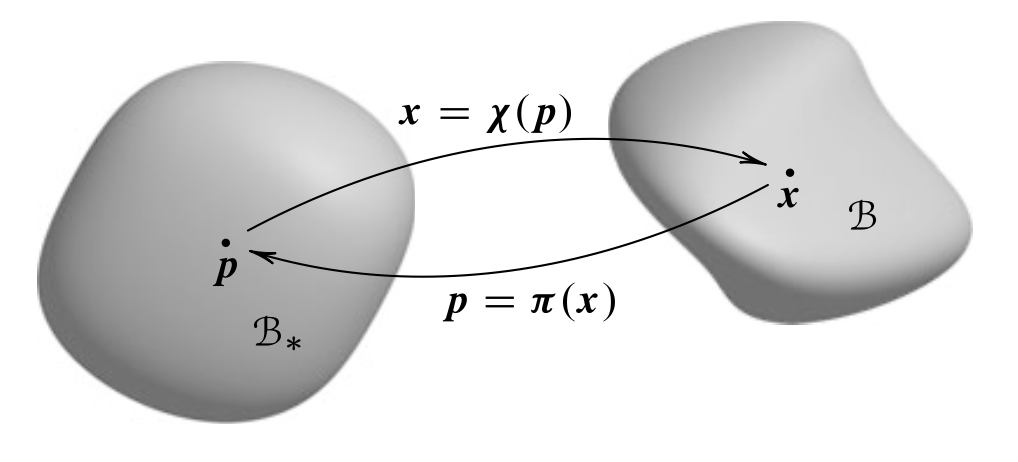
\includegraphics[width=0.8\linewidth]{images/def0}\ \ }
\end{Figure}

\textbf{Deformation gradient.} $F(p)=\nabla_{\!p}\chi$ such that
\begin{equation*}
\chi(q)=\chi(p)+F(p)[q-p]+o(q-p)
\end{equation*}

Fix origin and coordinate axes, $\de \underline{x}=F\,\de\underline{X}$ and component-wise it is
\begin{equation*}
F_{iK}=\frac{\partial x_i}{\partial X_K} 
\end{equation*}

Moreover, F can be seen as a linear trasformation
\begin{equation*}
F:T_{_X} \bt_*\to T_x \bt
\end{equation*}

\rule{0.31\textwidth}{0.2pt}
\smallskip

\textbf{Change of variables.} $\text{det}(F)=J>0$, then
\begin{align*}
\de V_x &= J\,\de V_{\!_X} \\
\underline{n}\,\de A_x &= JF^{\,\text{-}T}\underline{n}_*\,\de A_{_X}\quad(\text{Nanson})
\end{align*}

\rule{0.31\textwidth}{0.2pt}
\smallskip

\textbf{Homogeneous deformation.} When $F\in\text{Lin}^+$ is costant we have an homogeneous def. In addiction, if $q$ is a fixed point, then we have
\begin{equation*}
\chi(p)=q+F[p-q]
\end{equation*}
Moreover, if $F\equiv R\in \text{SO}(3)$ then we have a solid/rigid deformation.

\rule{0.31\textwidth}{0.2pt}
\smallskip

\textbf{Polar decomposition thm.} $\forall\,F\in\text{Lin}^+$ $\exists\,!$ $R\in\text{SO}(3)$, $U,V\in\!\text{Sym}^+$ st $F=RU=VR$.

\rule{0.31\textwidth}{0.2pt}
\smallskip

\textbf{Cauchy-Green tensors.} They are defined as
\begin{align*}
\text{left}\quad B&=FF^T=V^2 \\
\text{right}\quad C&=F^TF=U^2
\end{align*}

$B,C\in\text{Sym}^+$, $C$ \emph{lives} on $\bt_*$ and $B$ on $\bt$

\rule{0.31\textwidth}{0.2pt}
\smallskip

\textbf{Motion.} Simply, it's $\underline{x}=\chi(\underline{X},t)=\underline{x}(\underline{X},t)$, so
\begin{equation*}
F(\underline{X},t)=\nabla_{\!\! _X} \underline{x}(\underline{X},t)
\end{equation*}

\vspace{-1em}

\rule{0.31\textwidth}{0.2pt}
\smallskip

\textbf{Material and spatial gradient.} $\phi=\phi(\underline{x},t)$ spatial field, its spatial gradient is
\begin{equation*}
\nabla_{\!\!_x} \phi=\frac{\partial \phi}{\partial \underline{x}}
\end{equation*}

Instead, its material gradient is 
\begin{equation*}
\nabla_{\!\!_X} \phi_m=\frac{\partial \phi_m}{\partial \underline{X}}=\frac{\partial \phi_m}{\partial \underline{x}}\,\frac{\partial \underline{x}}{\partial \underline{X}}=\left( \nabla_{\!\!_x} \phi \right)_m \cdot F
\end{equation*}

formally, just $\boxed{\nabla_{\!\!_X} \phi=\nabla_{\!\!_x} \phi\cdot F}$

\rule{0.31\textwidth}{0.2pt}
\smallskip

\textbf{Velocity and acceleration.} They are
\begin{equation*}
\dot{\underline{x}}(\underline{X},t)=\frac{\partial\, \underline{x}(\underline{X},t)}{\partial t} \quad  \ddot{\underline{x}}(\underline{X},t)=\frac{\partial^2 \underline{x}(\underline{X},t)}{\partial t^2}
\end{equation*}

and $\underline{v},\underline{a}$ are the equivalent spatial representation.

\smallskip

The gradient of the material velocity is
\begin{equation*}
\nabla_{\!\!_{X}} \dot{\underline{x}}=\frac{\partial}{\partial \underline{X}} \frac{\partial\underline{x}}{\partial t}\overset{\scriptstyle\text{SW}}{=} \frac{\partial}{\partial t} \frac{\partial \underline{x}}{\partial \underline{X}}=\dot{F}
\end{equation*}

so formally, $\boxed{L:=\nabla_{\!\!x}\underline{v}=\dot{F}F^{\,\text{-}1}}$ 

\smallskip

By orthgonal decomposition for $2^{\text{nd}}$-rank tensor
\begin{equation*}
L=\frac{L+L^T}{2} +\frac{L-L^T}{2} =D+W
\end{equation*}

where $D\in\text{Sym}$ is the stretching tensor and $W\in\text{Skw}$ is the spin tensor.

\vspace{-0.5em}

\rule{0.31\textwidth}{0.2pt}
\smallskip

\textbf{Material and spatial time derivative.} $\phi$ spatial field, its spatial time derivative is
\begin{equation*}
\phi'=\frac{\partial \phi}{\partial t}
\end{equation*}

Instead, its material time derivative is 
\begin{equation*}
\left(\phi_m\right)^\cdot=\left(\phi'\right)_m+\left( \nabla_{\!\!_x} \phi \right)_m \cdot \dot{\underline{x}}
\end{equation*}

formally, just $\boxed{\dot{\phi}=\phi'+\nabla_{\!\!_x} \phi \cdot \underline{v}}$

\smallskip

Using this formula with $\phi\equiv \underline{v}$ we obtain
\begin{equation*}
\boxed{\underline{a}=\underline{v}'+ \left(\nabla_{\!\!_x}\underline{v} \right) \underline{v}}
\end{equation*}

\rule{0.31\textwidth}{1pt}












%!TEX root = ../main.tex

% =================================================

% \subsection{\color{red}Bho}

% =================================================
%!TEX root = ../main.tex

% =================================================

% \subsection{\color{red}Bho}

% =================================================

\end{multicols*}
\end{document}